\documentclass{sig-alternate}
\usepackage[T1]{fontenc}
\usepackage{array}
\usepackage{verbatim}
\usepackage{booktabs}
\usepackage{fancyvrb}
\usepackage{url}
\usepackage[english]{babel}
\usepackage{listings}
\usepackage{myref}
\usepackage{microtype}

%all of the following is for the todonotes package
\usepackage{marginnote}
\usepackage[textsize=tiny]{todonotes}
\renewcommand{\marginpar}{\marginnote}
\setlength{\marginparwidth}{1.8cm}
\setlength{\marginparsep}{0.1cm}
\newcommand{\zfc}[1]{\todo[color=green]{ZFC: #1}}
\newcommand{\mm}[1]{\todo[color=red]{MM: #1}}
\newcommand{\js}[1]{\todo[color=blue!30]{JS: #1}}
\newcommand{\clg}[1]{\todo[color=yellow]{CLG: #1}}
\newcommand{\someone}[1]{\todo[color=orange]{SOMEONE: #1}}
%end todonotes section%

\newcommand{\minisec}[1]{\vspace{2ex}\noindent\textbf{#1}}

\makeatletter
\makeatother

\begin{document}



\lstset{language=Java}
\definecolor{dkgreen}{rgb}{0,0.5,0}
\definecolor{dkred}{rgb}{0.5,0,0}
\definecolor{gray}{rgb}{0.5,0.5,0.5}
\lstset{
basicstyle=\ttfamily\bfseries\scriptsize,
  morekeywords={virtualinvoke}, 
  keywordstyle=\color{blue},
  ndkeywordstyle=\color{red},
  commentstyle=\color{dkred},
  stringstyle=\color{dkgreen},
  numbers=left,
  breaklines=true,
  numberstyle=\ttfamily\tiny\color{gray},
  stepnumber=1,
  numbersep=6pt,
  backgroundcolor=\color{white},
  tabsize=4,
  showspaces=false,
  showstringspaces=false,
  xleftmargin=.23in
}
%original settings on at least some of the figures: 
%\author{BLINDED FOR SUBMISSION}

\title{Evaluating the Flexibility of the Java Sandbox}

\numberofauthors{1} 
\author{\alignauthor Zack Coker, Michael Maass, Tianyuan Ding, Claire Le Goues, and Joshua Sunshine \\
\affaddr{Carnegie Mellon University} \\
\email{\{zfc,mmass\}@cs.cmu.edu, tding@cmu.edu, \{clegoues,sunshine\}@cs.cmu.edu}
} 

\maketitle
%JSS: This is to force page numbers.
\thispagestyle{plain} 
\pagestyle{plain}
\begin{abstract}
The ubiquitously-installed Java Runtime Environment (JRE) executes
untrusted code inside a sandbox to protect the host machine from potential
malicious behavior. However, dozens of recent exploits have successfully
escaped the sandbox, allowing attackers to infect numerous
Java hosts. It is essential to distinguish patterns of malicious use
from patterns of benign use to proactively prevent future exploits.
We therefore performed an empirical study of benign open-source Java
applications and compared their use of the sandbox to the usage present
in recent exploits. We found that benign applications with secured
sandboxes do not modify the security manager, the security policy
enforcement mechanism, after it is first set and do not attempt to
directly use privileged classes. Exploits routinely do both. We derive 
two rules from these results to prevent (1) security manager 
modifications and (2) privilege escalation. We evaluated their protection merits 
in a case study using runtime monitors to enforce the rules during the 
execution of exploits and benign applications. The rules stop all ten 
Metasploit Java 7 exploits without breaking backwards compatibility 
with benign applications. These practical rules should be enforced 
in the JRE to fortify the Java sandbox.
\end{abstract}

\section{Introduction}

\iffalse
\begin{figure}
\begin{centering}
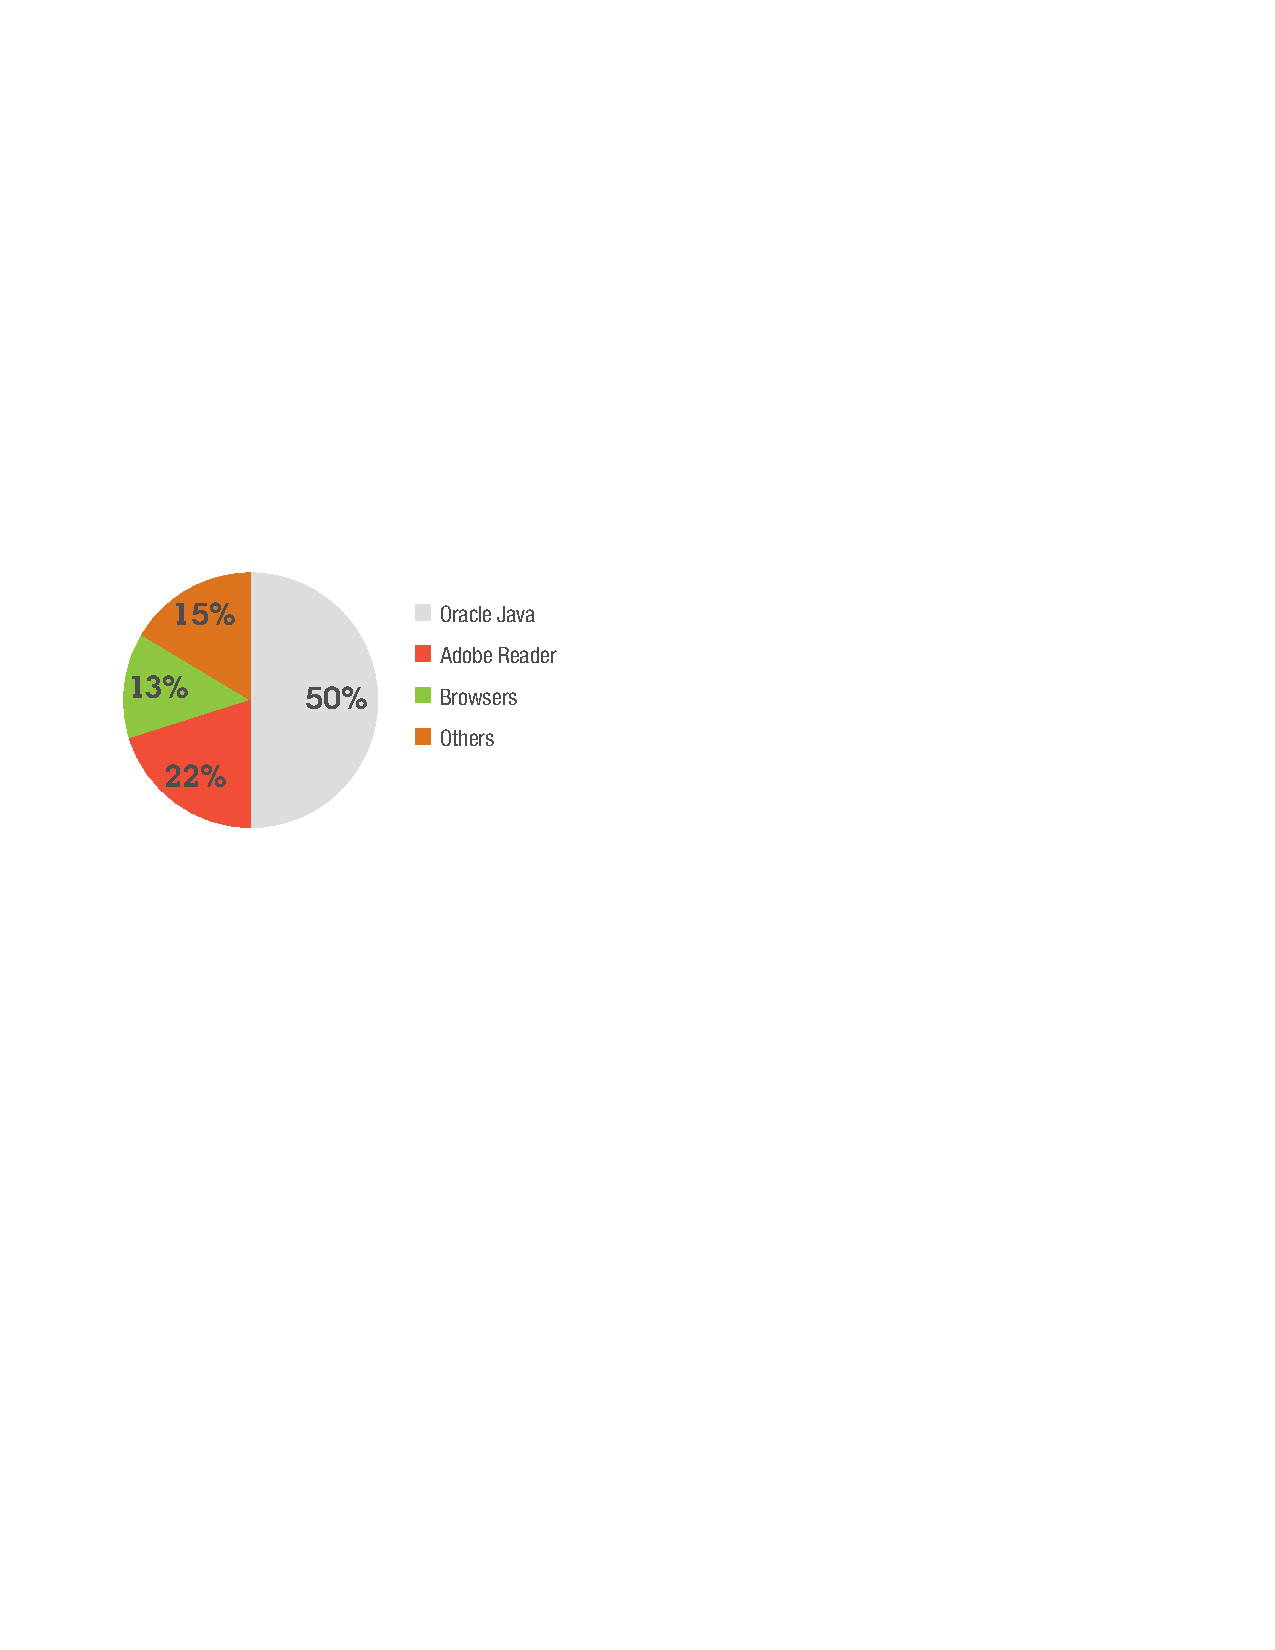
\includegraphics[width=2in]{most_targeted_apps_ibm_xforce}
\par\end{centering}
\caption{Pie chart showing the most
targeted applications on enterprise workstations, according to to
a Dec. 2013 survey of Trusteer customers \cite{xforceQ12013}. Java
\label{fig:most-targeted-applications}represented half of all attack-attempts in their sample.}
\end{figure}
\fi

Java is a popular target for attackers,
for three broad reasons.  First, the Java Runtime Environment (JRE) is widely installed on user endpoints.
Second, the JRE can (and often does) execute external code, in the form of
applets and Java Web Start (JWS) %~\cite{_java_web_start}
applications~\cite{gong1997going,gong2003inside}.  Finally, there are hundreds
of known and zero-day vulnerabilities (e.g. CVE-2013-0422)~\cite{xforceQ12013}
in Java. In the
common scenario, often referred to as a ``drive-by download'', attackers lure
users to a website that contains a hidden malicious applet. Such malicious
applets exploit security vulnerabilities in the JRE to deliver malware,
often leaving the user unaware.

In theory, such attacks should not be so common: 
Java provides a sandboxing mechanism that enables the safe execution of untrusted code and isolates
components from one another. Both the host application and machine should
therefore be protected from malicious behavior.
In practice, these security mechanisms are problematically
buggy, such that Java malware typically alters the sandbox's
settings~\cite{garber_2012} to override security mechanisms. Such exploits take advantage of defects in either
the JRE itself or the application's configuration of the sandbox to 
disable the security manager, the component of the sandbox responsible for enforcing the
security policy~\cite{fireeye_2013,svoboda_anatomy_blog_2013,security_explorations_2012,blackhat_2012}.
Many of these exploits contain similar behaviors\zfc{Probably should cite this;  If we like this version, I should ask Michael what to cite}.  

If we understood how benign applications interact with the sandbox, we could 
identify and prevent exploits.  Unfortunately, the Java sandbox is very 
powerful and flexible, possibly more flexible than intended, which means
many diverse interactions are possible.
Up to now, benign sandbox interactions were not 
understood in the research community.  Li Gong, the main designer of the 
Java security architecture, admitted in a ten year retrospective on Java 
Security that he didn't know how or how extensively the ``fine grained 
access control mechanism'' (i.e. the Java sandbox) is used~\cite{gong2009java}.  
Without this knowledge, any attempt to stop exploit behavior could stop 
safe applications.  And yet, there are also other advantages to be gained by 
understanding how developers use the sandbox.  Common developer problems 
could provide insight for designing similar solutions.  Unintended sandbox
uses could suggest the need for a new feature in the Java language.  

To explore these problems, we conducted an empirical study
to answer the question: How do benign
applications interact with the Java security manager?  We identified 36
open-source Java projects that use the security manager, taken from the Qualitas
Corpus \cite{QualitasCorpus:APSEC:2010} and GitHub, and characterized
those interactions. 

We came to find that some applications did not use the sandbox as intended.  Some
applications use the sandbox for non-security uses.  Others used questionable 
security methods to change the current security policies.  We hypothesis that 
these methods are the result of unnecessary complexity and flexibility
in the design and engineering of Java's security mechanisms.  For example,
applications are allowed to change the security manager at runtime, whereas 
static-only configuration of the manager would be more secure. The JRE also
provides a number of security permissions that are so powerful that an application
that uses one is essentially running without the protections of the sandbox, 
making the manager defenseless.
%In this paper, we investigate this disconnect between theory and practice.  We
%hypothesize that it results primarily from unnecessary complexity and flexibility
%in the design and engineering of Java's security mechanisms.  For example,
%applications are allowed to change the security manager at runtime, whereas 
%static-only configuration of the manager would be more secure. The JRE also
%provides a number of security permissions that are so powerful that an application
%that uses one is essentially running without the protections of the sandbox. We 
%hypothesize that benign applications do not need all of this power, and that
%they interact with the security manager in ways
%that are measurably different from the ways that exploitative applications do.  
%If true, this difference can be leveraged to improve the overall security of
%Java applications, and prevent future attacks.

We discovered two types of security managers in
practice. \emph{Defenseless} managers enforce a policy that allows sandboxed code
to modify sandbox settings. Such applications
are inherently insecure, because externally-loaded malicious code can
modify or disable the security manager.  In our study, defenseless managers were
used by applications that modified sandbox settings at runtime, typically because
they use the security manager to enforce policies or implement functionality
unrelated to security.  We believe that such applications use the
sandbox to implement certain non-security requirements
because Java does not provide better mechanisms for doing so.  
The sandbox is not intended to be used this way, and these use cases
effectively limit the potential exploit mitigations that are
backwards compatible with all benign applications. 
On the other hand, applications with \emph{self-protecting} managers do 
not allow sandboxed code to modify security settings. 
It might still be possible to exploit
such applications due to defects in the JRE code that enforces security
policies, but not due to poorly-deployed local security settings.


Overall, we found that the software that \emph{did} use the sandbox in
non-trivial, defenseless, or otherwise
unusual ways typically did so incorrectly or insecurely. In fact, we found and reported a
security vulnerability related to the sandbox in one of the applications under study. We also found that
software that uses the sandbox for its intended
purpose---protection from malicious external code---does not use its
vast flexibility.  For these applications, the flexibility decreases their security without
obviously benefiting the developers or application functionality.  We therefore propose 
two runtime rules that restrict the flexibility of the sandbox and fortify Java
against the two most common modern attack types without breaking backwards
compatibility in practice. We evaluate our rules
with respect to their ability to guard against ten applets in a popular exploit development 
and delivery framework, Metasploit
4.10.0%
\footnote{http://www.metasploit.com/}, that successfully attack unpatched
versions of Java 7. 
Taken together, the rules stopped all ten exploits, and did not break
backwards-compatability 
when tested against a corpus of benign applications.
We are engaged in an
ongoing discussion on the security-dev mailing list for OpenJDK about
implementing runtime enforcement of these rules in the JVM itself.

The contributions of this papers are as follows:
\begin{flushitem}	\setlength{\parskip}{0pt}
  \setlength{\parsep}{0pt}
  \setlength{\itemsep}{0pt}
\item A catalog of open-source applications that enforce constraints on
  sub-components by way of the Java sandbox (Section \ref{sec:Study-results}).
\item \todo{A study of how open-source applications interact with the security
    manager, with implications.}
\item An enumeration of Java permissions that make security policies difficult
  to enforce (Section \ref{sec:secmanagers}), a discussion of real-world cases
  where these permissions are used (Sections \ref{sub:Non-security-uses-of} and
  \ref{sub:Using-the-Security}), and a sandbox-bypassing exploit for a popular
  open-source application made vulnerable due to their use (Section
  \ref{sub:Using-the-Security}).
\item Two novel rules for distinguishing between benign and malicious Java
  programs, which we validated with an empirical evaluation (Section
  \ref{sec:Rules-for-Fortifying}).
\item A discussion of the various tactics for practically implementing the
  rules, with a case for adoption directly in the JVM (Section
  \ref{sub:Implementation-Using-JVMTI}).
\end{flushitem}

% This paper covers background on the Java sandbox and its exploits necessary to fully motivate and 
% understand this work in Section~\ref{sec:Background} before discussing our study's methodology and 
% dataset in Section~\ref{sec:Security-Manager-Study}. The results of the study are discussed in 
% Section~\ref{sec:Study-results}, leading to our rules which are defined and evaluated in 
% Section~\ref{sec:Rules-for-Fortifying}. Finally, we discuss the limitations of this work, cover 
% related work, and conclude in Sections \ref{sec:Limitations}, \ref{sec:related}, and 
% \ref{sec:Conclusion} respectively.

\section{Background}\label{sec:Background}

In this section, we describe the Java sandbox
(Section~\ref{sec:sandbox}), distinguish between defenseless and self-protecting
security managers (Section~\ref{sec:secmanagers}) and provide a high-level
description of how Java exploits commonly work
(Section~\ref{sec:javaexploits}). 

\subsection{The Java sandbox}
\label{sec:sandbox}

\begin{figure}
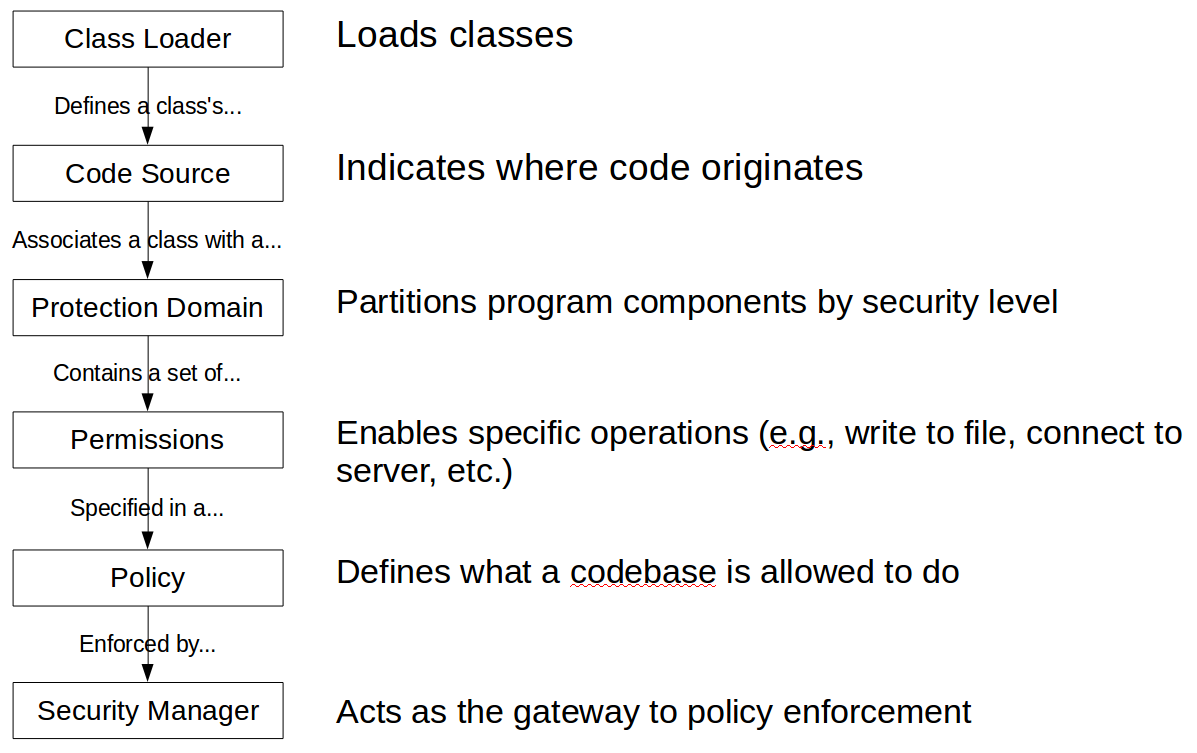
\includegraphics[width=\columnwidth]{sandbox_overview}
\caption{High-level summary of the components of the Java 
\label{fig:Sandbox-high-level-summary}
sandbox.}
\end{figure}

The Java sandbox is designed to safely execute code from untrusted
sources. 
The relevant components are summarized in Figure
\ref{fig:Sandbox-high-level-summary}. 
When a \textit{class loader} loads a class (e.g., from
the network, filesystem, etc.), it assigns the class a \textit{code source} that
indicates the code origin, and associates it with a \textit{protection
  domain}. Protection domains segment the classes into groups by
\textit{permission set}. These sets
contain permissions that explicitly allow actions with security
implications, such as writing to the filesystem, accessing the network, using
certain reflection features, etc~\cite{_permissions_2014}.  Unlisted actions are disallowed.
\emph{Policies} written in the Java policy
language~\cite{_java_policy_language} define the permission sets and the code
sources associated with them. 
By default, all classes \emph{not} loaded from the local file system are run
within a restrictive sandbox, with policies that restrict their ability to
interact with the host application or machine. 

The sandbox is activated by setting a \emph{security manager}, which acts as the
gateway between the sandbox and the rest of the application. Whenever a
sandboxed class attempts to execute a method with security implications, that
method queries the security manager to determine if the operation should be
permitted. 
To perform a permission check, the security manager walks the call stack to
ensure each class in the current stack frame has the specific permission needed to
perform the action.\footnote{Stack-based access control is discussed in more
  detail
  in~\cite{banerjee_stack-based_2005,besson_stack_2004,d._s._wallach_understanding_1998,erlingsson_irm_2000,fournet_stack_2002}}
  % ,pistoia_beyond_2007,zhao_type_2005}.}
% CLG unilaterally declares that we don't need this many references to help
% people look up/understand stack-based access control.

Missing checks in code that \emph{should} be protected are a common
source of Java vulnerabilities, because the security-critical code must initiate
the check.  Note that such vulnerabilities lie in the JRE itself (i.e., the code
written by the Java developers), not in code using the sandbox to
execute untrusted code.

\subsection{Defenseless vs. self-protecting managers}
\label{sec:secmanagers}

\begin{table*}
\caption{List of sandbox-defeating permissions. A security manager that enforces
a policy containing any of these permission results
\label{tab:defenseless-permissions}
in a defenseless sandbox. A subset of these permissions were first identified in \cite{security_explorations_2012}. 
}
\begin{tabular}{ll}
\toprule 
\textbf{Permission} & \textbf{Risk}\tabularnewline
\midrule
RuntimePermission(``createClassLoader'') & Load classes into any protection domain\tabularnewline
RuntimePermission(``accessClassInPackage.sun'') & Access powerful restricted-access internal classes\tabularnewline
RuntimePermission(``setSecurityManager'') & Change the application's current security manager\tabularnewline
ReflectPermission(``suppressAccessChecks'') & Allow access to all class fields and methods as if they are public\tabularnewline
FilePermission(``<\textcompwordmark{}<ALL FILES>\textcompwordmark{}>'',
``write, execute'') & Write to or execute any file\tabularnewline
SecurityPermission(``setPolicy'') & Modify the application's permissions at will\tabularnewline
SecurityPermission(``setProperty.package.access'') & Make privileged internal classes accessible\tabularnewline
\bottomrule
\end{tabular}
\vspace{-0.5cm}
\end{table*}

% \todo{I think we need to hammer this point a bit more: Java's security model is
%   too complicated---meaning it's implemented badly/in a way that's full of
%   bugs---and also unecessarily so---because people don't need all that
%   flexibility.  I'm not sure how to expand this text to help with that
%   point-hammering, but I think it would be useful to the development of the
%   argument.  Anyone see what I'm getting at and want to try to expand accordingly?}
Java is flexible about when in an application's execution the sandbox
is enabled, configured, and reconfigured. The default case for web applets and applications
that use Java Web Start is to set what we call a \textit{self-protecting} security
manager before loading the network application. The security
manager, and thus the sandbox, is self-protecting in the sense that
it does not allow the application to change sandbox settings. Self-protecting managers might
still be exploited due to defects in the JRE code that enforces security
policies, but not due to poorly-deployed local security settings.We contrast
self-protecting managers with those we call 
\textit{defenseless}, meaning that sandboxed applications are 
permitted to modify or disable the security manager.  
A defenseless manager is virtually useless in terms of improving the
security of either a constrained application or its host. However, we find
in Section~\ref{sec:Study-results} that developers
have found interesting non-security uses for defenseless managers in otherwise
benign software.

Table~\ref{tab:defenseless-permissions} summarizes the set of permissions
that distinguish between self-protecting and defenseless security
managers. We generated this list by evaluating whether each of the available Java permissions to
can \clg{what does ``reliably'' mean here? Can we drop it, or is it adding some
  important meaning?} reliably lead to sandbox bypasses. We
call any security manager that enforces a policy 
containing any of these permissions \emph{defenseless.}

\subsection{Exploiting Java code}
\label{sec:javaexploits}

\iffalse
\begin{figure}
\begin{centering}
\begin{lstlisting}[language=Java,basicstyle={\scriptsize}]
import java.lang.reflect.Method; 
import java.security.AccessController; 
import java.security.PrivilegedExceptionAction;   

public class Payload 
        implements PrivilegedExceptionAction {         
    public Payload() {
        try {
            AccessController.doPrivileged(this);
        } catch(Exception exception) { }     
    }

    public void run() {
        // Disable sandbox
        System.setSecurityManager(null);
    }

    public static void outSandbox() {
        // Do malicious operations
    }
}
\end{lstlisting}

\par\end{centering}

\caption{A typical sandbox-disabling  \label{fig:A-typical-exploit-payload}
Java exploit payload from http://pastebin.com/QWU1rqjf.}
% CLG isn't convinced that this figure is adding enough to justify the amount of
% space it's taking up.
% MM Would probably get rid of Fig 3 (Batik) first. This links to source
% code of what was an actual 0-day exploit, in its original form. This is %  the only place we directly reference such a thing for people who want
% to something really concrete.
\end{figure}
\fi

% Between 2011 and 2013, drive-by 
% downloads that used Java applets as the vector were widely reported.\todo{needs
%   a reference.  Also, I'm considering killing this sentence, but haven't decided
% yet.}
%
% This section provides an analysis of privilege escalation in the Java
% security model and recent Java exploits. 
While the Java sandbox \textit{should} prevent malicious applets from
executing their payloads, certain defects in the JRE implementation of these security mechanisms can permit
malicious code to set a security manager to \texttt{null}.  
This disables the sandbox, allowing
previously constrained classes to perform operations with the privileges of 
the JRE itself. 
This approach was taken in a large proportion of drive-by downloads exploiting
Java applets between 2011 and 2013~\cite{fireeye_2013}. 
%Figure \ref{fig:A-typical-exploit-payload}
%shows a typical payload class whose privileges have been elevated
%by an exploit to allow it to disable the sandbox. This example payload
%uses \texttt{doPrivileged} to allow the unprivileged exploit class
%to execute the operations in the payload without causing a \texttt{SecurityException}.
%

There are a couple of methods by which an exploit may nullify a security manager.
In \textbf{type confusion} attacks, an exploit breaks type
safety to craft an object that can perform operations as if it had
a different type.  Commonly, attackers craft objects that either
(1) point to the \texttt{System} class or (2) act as if they had
the same type as a privileged class loader (see CVE-2012-0507 \cite{_vulnerability_2012_0507}).
With the first approach, an attacker can directly alter (and disable) the
security manager; with the second, an attacker can load an exploitative
payload with elevated privileges.  In \textbf{confused deputy} attacks,
exploitative code ``convinces'' another 
class to return a reference to a privileged class~\cite{hardy_confused_1988}
known to contain a vulnerability (such as a missing security check).  The
attacker then takes advantage of that vulnerability to disable the sandbox 
(see CVE-2012-4681 \cite{_vulnerability_2012_4681}).
The ``convincing'' is necessary
because it is rare that a vulnerable privileged class is directly accessible
to all Java applications; doing so violates the \textit{access
control} principle that is part of the Java development culture.%
\footnote{\url{https://blogs.oracle.com/jrose/entry/the_isthmus_in_the_vm}%
} 

The confused deputy is an example of \emph{privilege escalation}.  Benign
applications rarely need to directly access privileged classes, and do not
typically have direct access to them anyway. 
Instead, the JRE provides less-privileged code path
to access these features. The danger of vulnerabilities in privileged
classes is therefore mitigated, because they cannot be directly exploited
unless malicious code first modifies its own privileges. 
This redundancy is implicit in the Java security model. % : If any class
% could load more privileged classes and directly execute
% of privileged operations, the sandbox in its current form would serve
% little purpose. 

In practice, however, Java's security mechanisms as implemented
in the JRE contains defects and vulnerabilities that reduce the benefits of
this redundancy.\footnote{Many of the recent type confusion and privilege escalation vulnerabilities
would not have been introduced if the JRE were developed strictly
following ``The CERT Oracle Secure Coding Standard for Java'' \cite{long_cert_2011,svoboda_anatomy_blog_2013,svoboda_anatomy_2014}}
  
Modern exploits that manipulate the Java security manager perform one
operation: They disable it.  This is possible largely because the Java security model
grants enormous flexibility to application developers to
set, reconfigure, manipulate, weaken, strengthen, or otherwise change a security
manager after it has been created.
Do applications need this power?  Do they regularly take advantage of the
ability to disable or weaken the sandbox? % If not, we can stop exploits for even currently unknown vulnerabilities by eliminating these operations without breaking backwards-compatibility with benign applications.
Our core thesis is that these security mechanisms are unecessarily
complex, and that the overall security of Java applications could be improved by
simplifying them, without loss to benign functionality.

\section{Security manager study}\label{sec:Security-Manager-Study}

In this section, we describe an empirical study consisting of static,
dynamic, and manual inspections of the open-source Java application landscape
that aims to understand the operations benign applications perform on the
manager. We focus our efforts on the security manager, as it is the
means by which applications interact with the sandbox.

Our basic research question is: How do benign open-source Java applications interact
with the security manager? The answer to this question informs which JVM-level
modifications can be used to improve security
while maintaining backwards compatibility.  The
possible mitigations vary in the strength with which they would be able to stop
potential exploits. 
% For example, a ``weak'' mitigation stops a small number of in-scope
% exploits and is easily bypassed.  An ``ideal'' mitigation stops all in-scope
% exploits and can never be bypassed.  
There are four possibilities:
\begin{flushenum}	\setlength{\parskip}{0pt}
  \setlength{\parsep}{0pt}
  \setlength{\itemsep}{0pt}
\item \textit{Benign applications never disable the security manager.}  If true,
  only exploitative code attempts to disable the security manager once it is set.
  The JVM could therefore eliminate an application's ability to
  do so.  This would be easy to implement, but would not guard against exploits
  that weaken the sandbox without disabling it.
% For example, attackers could potentially bypass the mitigation
% by modifying the enforced policy to allow the permissions they need
% or they could replace the current manager with one that never throws
% a \texttt{SecurityException}.
\item \textit{Benign applications do not weaken a set security manager}.  If
  true, the JVM could be modified to prevent any weakening or disabling of the 
  sandbox once it's set.  This is more powerful than simply removing the
  ability to disable the security manager, but is significantly more difficult to
  implement.
  % However, this would require the ability to
  % differentiate between changes that weaken the sandbox and those that do not,
  % a difficult problem.
  % Classifying changes in this manner autonomously is difficult
  % because it requires context specific information that a general mitigation
  % strategy may not have. 
  For example, if a permission to write to a file is
  replaced by a permission to write to a different file, is the sandbox
  weakened, strengthened, or exactly as secure as it was before?
\item \textit{Benign applications never modify the sandbox if a self-protecting
    security manager has been set}. If true, the JVM could be modified to
  disallow any change to a self-protecting security manager, defined by the
  policy it enforces.  This could be implemented with a simple runtime monitor that
  determines if a security manager is self-protecting (based on the permissions
  it sets) when an application
  attempts to change the sandbox. This is much easier to implement soundly than
  the previously-described approach, and guards against the same number and types of
  exploits.
  % This can
  % be easily achieved. While this mitigation has the same outcome as the moderate
  % mitigation, it is significantly easier to implement soundly and it is
  % therefore more likely to be effective in practice.
\item \textit{Benign applications do not change a set security manager.} If
  true, any attempted change to an already established security manager can be
  considered malicious. This would be the ideal result: restricting this
  operation is easy to implement in the JVM.
\end{flushenum}

This section describes our study dataset (\secref{Applications-Studied}) and
methodology (\secref{methodology}); we describe results in the next section
(\secref{Study-results}). 

\subsection{Dataset}\label{sec:Applications-Studied}

\begin{table}
\caption{Security manager interactions
  dataset.\label{Table:applications-studied}\clg{Whoops, we need lines of code
    on this, either in the table itself, or summarized in text (range, median
    size, total).}}
\begin{tabular}{lll}
\toprule 
Application Name & Description & Repo\tabularnewline
\midrule
(Apache) Ant & Java Project Builder & QC\tabularnewline
(Apache) Batik & SVG Image Toolkit & QC\tabularnewline
%C-JDBC & DB Cluster Middleware & QC\tabularnewline
%Compiere & Business Tools & QC\tabularnewline
(Apache) Derby & Relational Database & QC\tabularnewline
%DrJava & IDE & QC\tabularnewline
Eclipse  & IDE & QC\tabularnewline
FreeMind & Mind-Mapping Tool & QC\tabularnewline
Galleon & Media Server & QC\tabularnewline
(Apache) Hadoop & Distrib. Comp. Frwk. & QC\tabularnewline
Hibernate & Obj.-Rel. Mapper & QC\tabularnewline
%HyperSQL & SQL DB & QC\tabularnewline
JBoss & Application Middleware & QC\tabularnewline
JRuby & Ruby Interpreter & QC\tabularnewline
(Apache) Lucene & Search Software & QC\tabularnewline
(Apache) MyFaces & Server Software & QC\tabularnewline
NekoHTML & HTML Parser & QC\tabularnewline
Netbeans & IDE & QC\tabularnewline
OpenJMS & Messaging Service & QC\tabularnewline
Quartz  & Job Scheduler & QC\tabularnewline
QuickServer & TCP Server Frwk. & QC\tabularnewline
Spring Framework & Web Dev. Library & QC\tabularnewline
(Apache) Struts & Web Dev. Library & QC\tabularnewline
%(Apache) Tapestry & Web Dev. Library & QC\tabularnewline
(Apache) Tomcat & Web Server & QC\tabularnewline
Vuze & File Sharing App. & QC\tabularnewline
Weka & Machine Learning Algs. & QC\tabularnewline
(Apache) Xalan & XML Trans. Library & QC\tabularnewline
(Apache) Xerces & XML Parsing Library & QC\tabularnewline
AspectJ & Java Extension & GitHub\tabularnewline
%DemoPermissions & Spring Extension & Github\tabularnewline
driveddoc & Application Connector & GitHub\tabularnewline
%FileManager- & FTP Server & Github \\ FtpHttpServer\tabularnewline
Gjman & Development Toolkit & GitHub\tabularnewline
IntelliJ IDEA & IDE & GitHub\tabularnewline
%Jmin & Lightweight JDK & Github\tabularnewline
%MCVersion-Control & Minecraft Utility & Github\tabularnewline
%NGOMS & Business Tools & Github\tabularnewline
oxygen-libcore & Android Dev. Lib. & GitHub\tabularnewline
refact4j & Meta-model Prog. Frwk. & GitHub\tabularnewline
Security-Manager & Alt. Security Manager & GitHub\tabularnewline
Spring-Modules & Spring Extension & GitHub\tabularnewline
System Rules & JUnit Extension & GitHub\tabularnewline
TimeLag & Sound Application & GitHub\tabularnewline
TracEE & JavaEE Support Tool & GitHub\tabularnewline
Visor & Closure Library & GitHub\tabularnewline
\bottomrule
\end{tabular}
\end{table}

The goal of this study is to understand how benign open-source Java programs use
and interact with the security manager.  In the absence of an existing corpus of
applications that interact with the manager, we sought to construct a varied dataset.
We combined relevant subjects from 
the QualitasCorpus (QC) version 20130901~\cite{QualitasCorpus:APSEC:2010}, a 
collection of popular open source Java applications created for empirical
studies, and GitHub.
While QC contains 112 applications, we found only 24 applications interacted with 
the security manager.  To increase the size and diversity of the dataset (beyond
those that meet the QC inclusion requirements), we
added 12 applications from Github that interact with the security manager.\footnote{Applets, commonly
run in a sandboxed environment, would be natural study subjects.  However, we were unable
to find any benign applets that interacted with the security manager, likely
because of Java's strict restrictions on their behavior.}
 Table
\ref{Table:applications-studied} lists the 36 applications that comprise the
dataset.  Version numbers
and Git commit hashes are available in an online supplement.%
\footnote{https://github.com/SecurityManagerCodeBase/\\
ProjectsProfiles/blob/master/\\
projects list.xlsx}

We identified the applications in the full QC set that use the security
manager by searching for the keyword \texttt{SecurityManager} in the applications'
source code.  We performed a similar process on
GitHub, searching only Java files. We added the keywords
\texttt{System.setSecurityManager(} and \texttt{System.setSecurityManager(null)}
to the search to remove false positives and to find applications that disable the
manager, respectively. We picked the top seven applications from the results for each keyword,
removing manually-identified false positives and applications that were
already included in the QC set. We studied each GitHub program at its most
recent commit as of June 2014.

\subsection{Methodology}
\label{sec:methodology}

We performed a tool-supported manual inspection of the applications in our
dataset to group them
into qualitative, non-overlapping categories based on their interactions with the security 
manager. The first category includes applications that can or do
\emph{change a set security manager} over the course of execution.\clg{At what
  point in this process did we determine whether a set security manager was
  defenseless or self-protecting?}
If an application did not change the security manager, 
we looked to see if it set a single security manager 
during execution.  If so, it
was categorized as \emph{sets an immutable manager.}  If an
application interacted with a security manager that it did not set, 
then the application contains logic to adjust to different security settings.
We categorized any such application
as \emph{supports being sandboxed.}  Finally, we identified
applications that tested for particular security settings and modified execution
to conform or adapt accordingly.
For the final category, if a
program did not contain any interaction with the security manager in 
the main application, but did interact with it
in test cases, we categorized the
application as \emph{only interacts in unit tests.}  This final category
includes applications that modify the security manager in unit tests, because doing
so allows for testing the program against multiple security settings.

We created static and dynamic analysis tools
to assist in a manual inspection of each application's security manager
interactions. We created a 
FindBugs~\cite{hovemeyer_finding_2004} plugin that
uses dataflow analysis to identify security manager initialization and calls to \texttt{System.setSecurityManager}().
The dynamic analysis tool uses the Java Virtual Machine
Tool Interface (JVMTI) \cite{_jvmti}
to inspect the current state of Java applications and control
their execution. The dynamic analysis tool sets a modification watch
on the \texttt{security} field of Java's \texttt{System} class, which
stores the security manager object for the application.
% The watch prints out the class name, source file name, and line of
% code where any change to the field took place. A special notice is
% printed when the field is set to \texttt{null}. 

We split the dataset between two of the authors, who each analyzed
applications using the following steps:

\begin{flushenum}\setlength{\parskip}{0pt}
  \setlength{\parsep}{0pt}
  \setlength{\itemsep}{0pt}
\item Run \texttt{grep} on all Java source files in the application.
Output every line containing the keyword \texttt{SecurityManager}.
Manually inspect the lines in their original source code files to understand
how the application interacts with the sandbox.
\item Run the static analysis on retained applications. Manually inspect the
  returned code, focusing on initialization. 
\item Execute the application with the dynamic analysis using parameters
  informed by the previous steps, 
to verify conclusions.
\item Summarize operations performed
on the security manager and categorize accordingly.
\end{flushenum}

We undertook a pilot study where each author
independently inspected the same six applications and compared their
results. This ensured the two authors understood the analysis steps 
and produced consistent results.


\section{Study results}\label{sec:Study-results}

In this section, we describe the results of our empirical study of open-source
Java programs and how they interact with the security manager. 

\subsection{Summary of benign behaviors}\label{sub:Evaluation-of-the-hypotheses}


\begin{table}
\caption{Classification of application
  interactions \label{tab:Classification-of-Application}
with the security manager.}
\begin{tabular}{lrrr}
\toprule 
Type of Interaction & QC & GitHub & Total\tabularnewline
\midrule
1. Sets an immutable manager & 6 & 1 & 7\tabularnewline
2. Changes set manager & 5 & 3 & 8\tabularnewline
3. Supports being sandboxed & 10 & 3 & 13\tabularnewline
4. Interacts only in unit tests & 3 & 5 & 8\tabularnewline
%5. No interactions (false positive) & 5 & 5 & 10\tabularnewline
\bottomrule
\end{tabular}
\end{table}

Recall that in Section~\ref{sec:Security-Manager-Study}, we refined the
high-level research question---how do benign applications interact with the
security manager?---into four possibilities, and that the possible mitigations
required in each case varied by strength and complexity.  Revisiting those
possibilities with respect to our dataset, we found:
\begin{flushenum}\setlength{\parskip}{0pt}
  \setlength{\parsep}{0pt}
  \setlength{\itemsep}{0pt}
\item Benign applications \emph{do} sometimes disable the security manager.
  However, we found that such applications typically use a defenseless sandbox for
  non-security purposes; we discuss further below.

\item Several benign applications \emph{do} provide methods for the user to
  dynamically change the security policy or the manager in ways that can reduce
  the security of the sandbox.

\item Benign applications do \emph{not} change the
security manager if a self-protecting security manager has been set.  

\item Benign applications do sometimes change a set security manager.  We
  observed multiple applications that changed a set security manager.
\end{flushenum}

In terms of the four possible mitigation strategies,
only the third---a runtime monitor that blocks modifications to a self-protecting security manager---can
improve security without breaking benign behavior. 
Fortunately, this technique does not require complex, context-sensitive
information about whether a change to a policy weakens the sandbox or not. 

% We characterize each application in our dataset along one of four types, depending on how they
% interact with the security manager:
% (1) applications that set an immutable
% security manager, (2) applications that change a set manager during
% the program's execution, (3) applications that do not set or modify a
% security manager in production code but will interact with a manager if 
% one is set by the user or another application, and (4) applications
% that only interact with the manager in unit tests. 
% 
Table \ref{tab:Classification-of-Application}
summarizes our dataset based on the categories we described
in~\secref{methodology}. Eight applications eliminate one or more possible
mitigation, while the rest cannot cause backwards compatibility issues with any
of the potential JVM modifications. We will
not discuss Type 3 or 4 applications further, because their interactions with
the sandbox do not provide useful insights in terms of common benign security
behaviors. 

Of the four categories, Type 2 applications (\emph{Changes set manager}) are the
most interesting, because they make the most use of Java's flexible security
mechanisms.  We therefore focus  
on these applications in our discussion. A few Type 1\clg{Besides the few/3-4 we
  discuss below, what do the rest of the 7 do?  Just set a manager, call external code in a
  sandbox, and then move on?  Do they do it properly?}
applications (\emph{Sets an immutable manager}) also provide interesting insights into
benign sandbox interactions. We discuss applications that use the sandbox for
purposes that are not security related in Section~\ref{sub:Non-security-uses-of}
and applications that use the sandbox for its intended security purposes in
Section~\ref{sub:Using-the-Security}.
\clg{How many have defenseless vs. self-protecting managers?}

\subsection{Non-security uses of the sandbox}\label{sub:Non-security-uses-of}

\begin{figure}
\begin{lstlisting}[firstnumber=691]
System.setSecurityManager(new AntSecurityManager(originalSM, Thread.currentThread()));
\end{lstlisting}
\vspace{-0.3cm}
\begin{lstlisting}[firstnumber=703]
// ...execute Ant...
\end{lstlisting}
\vspace{-0.3cm}
\begin{lstlisting}[firstnumber=723]
finally {
  // ...
  if (System.getSecurityManager() instanceof AntSecurityManager) { 
      System.setSecurityManager(originalSM); 
  }
\end{lstlisting}\vspace{-0.3cm}
\caption{Snippet of Eclipse code that uses a security manager to prevent Ant\label{fig:Eclipse-snippet}
from terminating the JVM.}
\end{figure}

Most of the applications to interact with the sandbox in
non-security ways did so to enforce architectural constraints when interacting with
other applications; the rest forcibly disabled the sandbox to reduce development
complexity. These applications provide insights into cases that are currently
hard for Java developers to handle without abusing security features. This abuse
of security features increases the difficultly of mitigating attacks against
them by increasing the odds of backwards compatibility issues.\clg{Are these
  type 1 or 2 applications?  Do they all require defenseless managers?}

\subsubsection{Enforcing architectural constraints}

Java applications often call \texttt{System.exit()} when a non-recoverable
error occurs. This can be a problem when the application in question is 
used as a library: The \texttt{System.exit()} closes the calling
application as well, because both applications
are running in the same JVM. 
To prevent this outcome without modifying the library application,
the calling application needs to enforce the architectural constraint
that called library code cannot terminate the JVM. 

We found three applications in our dataset that 
enforce this constraint by setting a security manager
that prevents \texttt{System.exit()} calls:
Eclipse, GJMan, and AspectJ.\footnote{%
GJMan contains a code comment referencing a
blog post that we believe is the origin of this solution. \url{http://www.jroller.com/ethdsy/entry/disabling_system_exit}}
For example, Eclipse uses Ant as a library.  Ant calls \texttt{System.exit()} to
terminate a currently-running build script in the event of an unrecoverable
error.  However, when Eclipse uses Ant as a library, it
should instead continue to execute, and report an error to the user.
Figure~\ref{fig:Eclipse-snippet} shows
how Eclipse sets a security manager to enforce this constraint
before executing Ant. After Ant closes and any error conditions
are handled, Eclipse restores the original manager.

This technique does enforce the
desired constraint, and appears to be the best solution available
in Java at the moment.  However, it is problematic for applications that also 
use the sandbox as intended, for security purposes.\clg{On reread, this isn't obvious to
  me.  The applications calling library code don't care about whether they're
  sandboxed, right?  Isn't it more a problem for people (or other programs) who want to run these
  applications in a sandbox? }  The technique requires
the application to dynamically change the security manager, which in turn requires a
defenseless manager.  As a result, the calling applications \emph{themselves} cannot be
effectively sandboxed, as might be desirable when run from Java Web Start, for
example. The host machine may thus be protected from code from the particular
sandboxed libraries, but not from vulnerabilities in the application itself, or
in library code that the application calls without a custom security manager.
\clg{Someone please check that the sentences I added/modified here are true.}

\subsubsection{Web applications outside the sandbox}\label{sub:Reducing-Web-Application-Complexity}

We also found applications that were complicated by the Java security policies
for web applications (applets~\clg{I thought we didn't study applets?} and applications launched via JWS). By default,
Java executes such applications inside a self-protecting 
sandbox with a restrictive policy that excludes
operations like accessing local files, retrieving resources
from any third party server, or changing the security manager. 

Applications in our set that cannot run without these permissions
opted to run outside of the sandbox.  
We found two applications that do this: Eclipse and
Timelag.  Both applications attempted
to set the security manager to \texttt{null} at the beginning of execution.
A restrictive sandbox catches this as a security violation and terminates the
application; to run it, the user must ensure that such a sandbox is not set.
The rationale for disabling the manager in Eclipse is explained in a 
code comment that reads, ``The launcher to start eclipse using webstart. To use
this launcher, the client must accept to give all security permissions.'' Timelag
performs the same operation, but without associated explanatory comments that we
could find, thus we can only 
infer developers motivation. 

The alternative to this method is to painstakingly
construct the application to run reasonably without required privileges (e.g. by
detecting the sandbox and avoiding or disabling privileged operations). To avoid executing
the applet\clg{again, I thought we weren't studying applets?} in a restrictive \clg{Actually, wouldn't Eclipse need to be run
  outside the sandbox anyway, because of the story with Ant from the previous subsection?}
sandbox, a developer must get the application digitally signed
by a recognized certificate authority, and then specify that the application should
run outside of the sandbox. 

\subsection{Using the security manager for security}
\label{sub:Using-the-Security}

This section describes applications that interact with the manager in
security-oriented ways.  Several of these applications eliminate all of the possible
JVM modifications that we consider do not consider if the manager is self-protecting.  Batik,
Eclipse, and Spring-modules provide 
methods that allow the user to set and change an existing manager. 
Ant, Freemind, and Netbeans explicitly set then change the manager.

Batik SVG Toolkit allows users to optionally constrain the execution of an application
that uses it by providing a method to turn the sandbox on or off. 
\clg{Confused.  How can a toolkit/library control the security of an application that
  uses it?  Can't it only constrain code that calls it?  I think I'm missing
  something here.}
This method
not only requires a defenseless sandbox, it provides a trivial mechanism for
disabling the sandbox at any time. The Batik download page
provides several examples of library use, one of which (the
``rasterizer'' demo) enables and disables the sandbox.  However, there seems to
be no reason to do so in this case other than to demonstrate the functionality;
we were otherwise unable to discern the rationale behind including it from the examples
and related documentation.

%  Two examples set
% a security manager at start up: the squiggle browser demo and the
% rasterizer demo. While the squiggle browser demo sets a manager and
% never changes it, the rasterizer demo calls \texttt{enforceSecurity}
% with a true argument the first time and a false argument the second
% time, which enables then disables the sandbox. While this was an interesting
% occurrence, there seems to be no valid reason to disable the sandbox
% in this case other than to show off the capability to do so.


\begin{figure}
\begin{lstlisting}[language=XML,basicstyle={\scriptsize}]
<permissions>   
  <grant class="java.security.AllPermission"/>   
  <revoke class="java.util.PropertyPermission"/> 
</permissions>
\end{lstlisting}
\caption{An example from Apache of an Ant build script element that grants all but
  one permission to external code. The resulting permission set results in a defenseless security
  manager (because it allows most of the permissions we list in
  Table~\ref{tab:defenseless-permissions}).  Revoking the
  \texttt{PropertyPermission} therefore does not improve the security of the
  application over running without the sandbox.} 
\label{fig:Ant Permissions Example}
\end{figure}

Ant, Freemind, and Netbeans all set then change the manager
at various runtime points.  As a result, we cannot entirely restrict the sandbox's
flexibility (by eliminating the ability to reconfigure, disable, or weaken it
at runtime) while maintaining backwards compatability with these applications.
Ant allows users to create scripts that 
execute \clg{external? User-provided?} Java classes under a user-specified
permissions set. Figure~\ref{fig:Ant Permissions Example}
shows an example permission set from the Ant Permissions website.%
\footnote{https://ant.apache.org/manual/Types/permissions.html%
} The contents of the \texttt{grant} element provide the application
all permissions; the \texttt{revoke} element then restricts
the application from using property permissions. However,
\texttt{PropertyPermissions} are not the only permissions that allow
malicious code to bypass or disable the sandbox (see
Table~\ref{tab:defenseless-permissions}).  The resulting security manager in this
example is thus defenseless.  This property set will still allow 
malicious code to perform all security-sensitve actions,
including those requiring \texttt{PropertyPermissions}, because the constrained
code is able to set or disable the security manager at will.\clg{Does the
  documentation surrounding this example on the website suggest that it's a good
  permissions set?}

When Ant prepares to execute an external, constrained class, it saves the
\clg{To be clear, this is separate from the behavior described above, right?  Oh
wait no, maybe not...but the example above is bad because it suggests to the
user that the permissions set is good, right?}
current security manager and replaces it with a custom manager. The custom
manager is not initially defenseless given a self-protecting permission set, but
it contains a private switch to make the manager defenseless for the purposes of
\clg{Why does it need to be made defenseless to restore the original manager?
  Doesn't Ant have the ability/permission to reset its own security manager
  after the constrained code is executed?}
restoring the original manager. With this implementation, Ant catches
applications that perform actions 
restricted by the user while typically protecting sandbox settings. 
%However, it
%is not clear this implementation 
%is free of vulnerabilities. 
% CLG believes this sentence is problematically speculative and could be said
% about basically anything.
Netbeans similarly sets a security manager around a separate application. 

Both of these cases require that the host application be run with a defenseless security manager, otherwise
the application would not be able to change the current security manager.
A better implementation would use a custom class
loader to load the untrusted classes into a constrained protection
domain. This approach would align with the intended usage of the sandbox.
Additionally, it would be more clearly correct and trustworthy while
allowing Ant and Netbeans to run inside of a self-protecting sandbox.
\clg{We speculate that they don't because it's hard or poorly understood?}

In trying to solve a similar problem, Freemind 0.9.0 illustrates
the dangers of a defenseless manager. Freemind is a mind mapping tool.  It
includes a feature that allows users to execute Groovy scripts on mind maps. 
The scripts are written by the creator of the mind map in question.
Groovy is a scripting language built on top of the JRE; typically, and in this
case, Java applications executing such scripts do so in the same 
JVM as the application itself. If the Groovy scripts are executed insecurely, it
may therefore be possible to exploit unsuspecting users by compelling them to download
a map and run its (malicious) scripts.

\begin{figure}
\begin{lstlisting}[language=Java,firstnumber=31]
/** By default, everything is allowed. But you
 * can install a different security controller
 * once, until you install it again. Thus, the
 * code executed in between is securely
 * controlled by that different security manager.  
 * Moreover, only by double registering the
 * manager is removed. So, no  malicious code 
 * can remove the active security manager.  
 * @author foltin */
public void setFinalSecurityManager(SecurityManager pFinalSM) {
  if(pFinalSM == mFinalSM){
    mFinalSM = null;
    return;
   } 		
   if(mFinalSM != null) {
     throw new SecurityException("There is a SecurityManager installed already."); 		
   } 		
   mFinalSM = pFinalSM;
 }	
\end{lstlisting}
\caption{Initialization of the field in Freemind's custom security
  manager\label{fig:Freemind-Security-Manager} that stores the proxy security
  manager. This demonstrates two problems with the current sandbox, as used by developers: (1) 
  using Java policies as a blacklist is
  dangerous and (2) modifying the manager at runtime requires 
  a work-around (ineffective or incomplete, in this case) to defend against malicious
  users. These problems were fatal to the security of this application.}
\end{figure}

This feature is implemented in Freemind within an architecture that
\emph{should} allow the
sandbox to enforce a stricter policy on the Groovy scripts than on
the rest of Freemind. 
Figure~\ref{fig:Freemind-Security-Manager} shows how Freemind sets
the proxy security manager field, a key component of this architecture.
%
The design centers around a custom
security manager that is set as the system security manager in the usual way.
This custom manager contains a field that holds a proxy manager, used only during the execution of
scripts. All checks to the security manager are 
deferred to this proxy manager.  As a result, if
the proxy field is set to \texttt{null}, the sandbox is disabled,
even though the system's manager is still set to the custom manager.
\clg{I'm a little puzzled by the code/explanation, so let me check my
  understanding.  If I'm reading this right,
  we're saying that if an exploit sets the proxy manager to null while
  the custom manager is in use and thinks that we're running a groovy script, it
  will defer checks to this proxy manager, which will do nothing.  Which is
  bad.  Am I wrong?}

As shown in Figure~\ref{fig:Freemind-Security-Manager},
once a manager is set, if \texttt{setFinalSecurityManager} is called
again with a different security manager, it throws a \texttt{SecurityException}.
Calling the method with a reference to the set manager disables
the sandbox.\clg{It's possible that this is the part that's confusing me.  Why
  do they do this/what does it accomplish?}
The comment implies that this approach is intended 
to prevent malicious applications from
changing the sandbox settings.

The code responsible for actually initiating the execution of the Groovy scripts
sets a proxy security manager that does not allow unsigned scripts to create
network sockets, access the file-system, or execute other programs. However,
despite all this security-oriented effort, the manager explicitly allows all
other permissions (including some that result in a defenseless sandbox) by
overriding the remainder of the permission check methods with implementations
that do nothing. As a result, a malicious script can turn off the sandbox at any
point.

However, the problem goes beyond the problematic permission checks overrides, and fixing
them would not result in the secure execution of untrusted Groovy scripts.  We
demonstrate this by using reflection to remove the custom security manager. 
Figure~\ref{fig:Example-Exploit-for-Freemind} 
shows a Groovy exploit that gets a reference to the system's manager
and its class. The class has the same type as the custom security
manager, thus the exploit also has access to a reference to the proxy manager field.
The exploit makes the field public and then reflectively sets it to
\texttt{null}, which disables the sandbox (since during script execution, all
checks are deferred to the proxy) and allows all
``forbidden'' operations.

We sent a notice to the Freemind developers in August, 2014
with our example exploit and advice on achieving
their desired outcome. Blu-ray player vendors have also introduced fatal
security flaws when attempting to execute some Java code with a stricter policy
than the rest of the system in unconventional ways, but we do not discuss these
cases because they are not
open-source.\footnote{\url{https://www.nccgroup.com/en/blog/2015/02/abusing-blu-ray-players-pt-1-sandbox-escapes/}} 

\begin{figure}
\begin{lstlisting}[language=Java,basicstyle={\scriptsize},breaklines=true]
def sm = System.getSecurityManager() 
def sm_class = sm.getClass() 
def final_sm = sm_class.getDeclaredField("mFinalSecurityManager")
final_sm.setAccessible(true) 
final_sm.set(sm, null)
new File("hacked.txt").withWriter { out -> out.writeLine("HACKED!") }
\end{lstlisting}
\caption{Exploit that breaks out of the scripting sandbox in Freemind\label{fig:Example-Exploit-for-Freemind}
to execute arbitrary code.}
\end{figure}

All of these applications ran afoul of the Java sandbox's flexibility even
though they attempted to use it for its intended purpose.\clg{What's wrong with
  Netbeans? I get that Ant provides bad examples to its users, but we barely
  discussed NetBeans.}  
They must all be run with defenseless managers, and those that 
manipulate the set security policy dynamically do so problematically.  
% Every application
% discussed in this section would break any of our suggested mitigations that do
% not check for self-protecting managers and can have executions protected by an
% easily bypassed, defenseless security manager. 
% CLG doesn't understand this sentence hopefully the gist is still maintained in
% the text here.
While Java does provide the
building blocks for constraining a subset of an application with a policy that
is stricter than what is imposed on the rest of the application, it is clear
that it is too easy to get this wrong:  We've seen no case where this goal was
achieved in a way that is known to be free of vulnerabilities.  \clg{I think
  this claim is strong.  What's wrong with Ant besides the bad example online?
  We didn't find a vulnerability in it, what kind of evidence do we require that
  their approach is secure?} These case
studies support our general claims that the Java security mechanisms are overly
complex, and that this complexity contributes to security vulnerabilities in
practice.  

\section{Fortifying the sandbox}
\label{sec:Rules-for-Fortifying}

Based on our study of how open-source Java programs interact with the security
manager, we propose two rules to stop Java exploits
from disabling the manager in applications that set a \emph{self-protecting}
security manager.  These rules reduce the flexibility and thus complexity of the
Java security model without breaking backwards compatability in practice:

\noindent\textbf{Privilege escalation rule.} If a self-protecting
security manager is set for the application, a class may not directly
load a more privileged class. This rule is violated when the protection
domain of a loaded class implies a permission that is not implied
in the protection domain that loaded it. About half of the exploits in the Metasploit set we use in our evaluation
break this rule to elevate the privileges of their payload
class.

\noindent \textbf{Security manager rule.} The manager cannot
be changed if a \emph{self-protecting} security manager has been set
by the application. This is violated when code causes a change
in the sandbox's configuration, the goal of many exploits.

%\subsection{Validating the Rules}\label{sec:Mitigations}

%In Section \ref{sec:Security-Manager-Study}, we discussed four hypotheses about security manager usage in benign applications, each
%of which, if validated, leads to a distinct mitigation. In Section
%\ref{sec:Study-results}, we gave empirical evidence in support of
%Hypothesis 3 and rejected all of the others. Along the way, we learned
%practical lessons about how applications use the Java sandbox that
%are useful to exploit mitigation implementers. 

In this section, we evaluate the protection merits and backwards compatibility
of these rules through an implementation of runtime monitors that
enforce them. This evaluation was done in collaboration with a large aerospace
company.
Section~\ref{sub:Implementation-Using-JVMTI} discusses how we implemented
our runtime monitors using JVMTI. Sections~\ref{sub:Effectiveness-at-Fortifying} and~\ref{sec:backcompat} explain the methodology behind and results of experiments we conducted
to determine how effective the rules are at stopping existing exploits without
breaking benign applications. 

\subsection{Implementation using JVMTI}\label{sub:Implementation-Using-JVMTI}

JVMTI is a native interface that enables the creation of
dynamic analysis tools, called agents, such as profilers, debuggers, monitors, and thread
analyzers. JVMTI agents can intercept and respond to events such as class
or thread creation, field access or modification, breakpoints, etc.

Our agent\footnote{Our agent is open-source. The latest version
of the tool can be found at https://github.com/SecurityManagerCodeBase/
JavaSandboxFortifier} must intercept three events to enforce the Privilege Escalation
and Security Manager rules: \texttt{ClassPrepare}, \texttt{FieldAccess},
and \texttt{FieldModification}. Enforcement of these rules is discussed in subsections \ref{sub:Enforcing-the-Privilege} and \ref{sub:Enforcing-the-SecurityManager}.

The field events require JVMTI to turn off the just-in-time compiler (JIT), which slows down program
execution enough that our monitors are not suitable for adoption on their
own. JVMTI implementations can avoid this limitation, but avoidance would likely
increase implementation complexity beyond what is reasonable for a diagnostic
interface. The right way to reduce this overhead is to embed our 
rules directly into the Java Runtime Environment.  We are currently in communication 
with the OpenJDK developers on their security-dev mailing list regarding enforcement of our rules in the JVM. 

\subsubsection{Enforcing the privilege escalation rule}\label{sub:Enforcing-the-Privilege}

The Privilege Escalation rule is enforced by ensuring that classes
can only load or cause the loading of more privileged classes in restricted-access
packages after a self-protecting security manager has been set. \textit{Restricted-access
packages} are packages that are public but not intended to be directly
used by typical Java applications; they are meant for internal JRE
use only. These packages are listed in the \texttt{package.access}
property in the \texttt{java.security.Security} class. There are two
ways to unsafely and directly access packages listed in this property:
(1) exploit a vulnerability in a class that can access them or (2)
allow access via the \texttt{accessClassInPackage} permission, which would lead to a defenseless manager if the named package is the \texttt{sun} package.

Benign applications can and often do use JRE classes to access these implementations by
calling restricted access package
classes (e.g., many of the classes in the \texttt{java.lang.reflect}
package are backed by classes in the restricted-access \texttt{sun} package, which
contains the internal implementations
for many Java features). We must therefore allow the JRE to load restricted-access packages
at runtime, while preventing such loading from the application classes.
Because exploit payloads are not implemented in restricted-access JRE packages,
the Privilege Escalation rule can permit this standard behavior while preventing
attacks.

To enforce the rule, our agent registers for
the \texttt{ClassPrepare} event, which allows the agent to inspect
a class after it is fully loaded but just before any of its code is
executed. Assuming the loaded class is not in a restricted-access
package, the agent inspects the stack frame to determine which class
caused the new class to be loaded. The agent must then get the protection
domains for both classes to ensure the loaded class is not more privileged by comparing their permission sets.

\subsubsection{Enforcing the security manager rule}\label{sub:Enforcing-the-SecurityManager}

The SecurityManager rule is enforced by monitoring every read from
and write to the \texttt{security} field of the \texttt{System} class.
This field stores the security manager.
The agent implements the read and write monitors by registering
\texttt{FieldAccess} and \texttt{FieldModification} events for the field. We 
monitor the field directly instead of instrumenting its getter and setter
methods to protect against type confusion attacks. 

The agent stores a shadow copy of the most recent security
manager. This copy is checked and updated via the JVMTI \texttt{FieldModification} event.
Whenenver the \texttt{security} field is written, the agent checks its
shadow copy of the manager.  If it is \texttt{null},
the manager is being set for the first time; the agent therefore checks
if the new manager is self-protecting. If so, 
the agent updates the shadow copy. If not, the agent stops performing stringent checks because the rule does not apply in the presence of a defenseless
manager. In either case, any further changes to the manager are logged.

The agent also registers and checks modifications to the field via
\texttt{FieldAccess} events, 
because the \texttt{FieldModification} event will not be triggered
when the manager is changed due to a type confusion attack.  Type confusion attacks
masquerade a malicious class as the
\texttt{System} class.  The masqueraded copy will have different internal
JVM identifiers for the class itself and its methods as compared to the legitimate
\texttt{System} class. However, because \texttt{System} is static, updating a
field in the masqueraded copy modifies the value in the legitimate copy. 
The
modification and access events are registered for specific field and
class identifiers, thus the events are not triggered for operations
on the malicious version. We leverage the mismatch this causes between
the set security manager and our shadow copy by checking if
the manager that is read has the same internal
JVM reference as our shadow copy every time a permission is checked. When the two references do not match,
the manager has been changed at some earlier point by a malicious class masquerading as
\texttt{System}. Type confusion attacks may also be used to masquerade
a class as a privileged class loader to elevate the privileges of
a payload class that disables the manager. This scenario is detected
by the modification event when the manager is disabled, but the type confusion attack would not be detected.


\subsection{Effectiveness at fortifying the sandbox}\label{sub:Effectiveness-at-Fortifying}

%%Need to integrate backwards-compatibility experiment here and mention proprietary applications tested through aerospace collaborator.

To evaluate our rules' ability to 
block sandbox-disabling exploits, 
we ran ten Java 7 exploits for the browser from Metasploit 4.10.0, an exploit development and delivery framework, on 64-bit
Windows 7 against the initial release of version 7 of the JRE.
Metasploit contains many Java exploits
outside of the subset we used, but the excluded exploits either only
work against long obsolete versions of the JRE or are not well positioned
to be used in drive-by downloads. 

We ran the ten exploits under the following conditions:
(1) without the agent, (2) with the agent but only enforcing the Privilege
Escalation rule, and (3) while enforcing both rules. We tested the Privilege
Escalation rule separately from the Security Manager rule because the latter
stops all of the exploits on its own. The Privilege Escalation rule is also worth validating on its own because it stops exploits earlier than the Security Manager rule and because it can detect attacks that are not targeting the manager. All  
ten of the exploits succeeded without the agent. Four
were stopped by the Privilege Escalation rule. All ten were stopped
when both rules were enforced. The exploits that were not stopped
by the Privilege Escalation rule were either type confusion exploits
or exploits that did not need to elevate the privileges of the payload
class. The payload class does not need elevated privileges when it
can directly access a privileged class to exploit. Table~\ref{tab:Exploit-experiment-summary}
summarizes our results, which show that together the rules are capable of stopping current exploit tactics while further narrowing available tactics in the future by blocking off privilege escalation routes.

\begin{table}
\caption{Effectiveness\label{tab:Exploit-experiment-summary} test results.}
\begin{tabular}{l>{\raggedright}p{3cm}l}
\toprule 
\textbf{CVE-ID} & \textbf{Privilege Escalation Monitor} & \textbf{Both Monitors}\tabularnewline
\midrule
2011-3544 & Attack Succeeded  & Attack Blocked\tabularnewline
2012-0507 & Attack Blocked & Attack Blocked\tabularnewline
2012-4681 & Attack Succeeded  & Attack Blocked\tabularnewline
2012-5076 & Attack Succeeded  & Attack Blocked\tabularnewline
2013-0422 & Attack Blocked & Attack Blocked\tabularnewline
2013-0431 & Attack Blocked & Attack Blocked\tabularnewline
2013-1488 & Attack Succeeded  & Attack Blocked\tabularnewline
2013-2423 & Attack Succeeded  & Attack Blocked\tabularnewline
2013-2460 & Attack Blocked & Attack Blocked\tabularnewline
2013-2465 & Attack Succeeded  & Attack Blocked\tabularnewline
\bottomrule
\end{tabular}
\end{table}

\subsection{Validating Backwards-Compatibility}\label{sec:backcompat}
\begin{table*}
\caption{\label{tab:validation-programs}
Backwards compatibility dataset.}
\centering

\begin{tabular}{lllll}
\toprule 
\textbf{Name} & \textbf{Description} & \textbf{KLOC} & \textbf{Number of Test Cases} & \textbf{Latest Commit}\tabularnewline
\midrule
ArgoUML & UML Tool & 389 & 1244 test cases & 1/11/15 \tabularnewline
Costello & GUI Testing Frontend & closed source & 9 provided examples & 5/09/12 \tabularnewline
CrossFTP & FTP Client & closed source & GUI fuzzing, sample workload & 1/18/15 \tabularnewline
JavaOpenStreetMap & Map Editor & 343 & 406 test cases & 1/18/15 \tabularnewline
JabRef & Reference Manager & 148 & 3 provided examples & 3/11/14 \tabularnewline 
mucommander & File Manager & 106 & 27 test cases & 1/23/14 \tabularnewline
\bottomrule
\end{tabular}
\vspace{-0.5cm}
\end{table*}

We validated that our rules are backwards compatible with benign applications by
attaching our monitors to executions of each application in
table~\ref{tab:validation-programs}. We chose to validate the rules using a dataset different from the one used in our earlier study. The new set is entirely composed of benign JWS applications that are automatically sandboxed in ways similar to applets, while the study's set contained many desktop applications. More importantly, the new dataset helps us ensure that our conclusions are not over-fitted to the study's set. In the new set, ArgoUML, JavaOpenStreetMap, and mucommand
contained unit tests that we ran in the presence of our monitors. Costello, and
JabRef did not contain tests, but did come with example workloads that we used
instead. CrossFTP contained neither tests nor sample workloads, thus we fuzzed
the GUI for 30 minutes using a custom fuzzer and uploaded a file to a remote FTP
server as a sample workload.\footnote{The GUI fuzzing source code can be found at \url{https://github.com/SecurityManagerCodeBase/GUITest/blob/master/RunGUITest.java}.}

In each case we confirmed that the tests, sample workloads, or fuzzed executions
worked without a security manager. To run the applications locally with the sandbox, we developed security
policies for each using a custom security manager that does not throw exceptions and that prints out checked permissions as each program executes. Finally, we ran each case a third time
using our policy and the standard Java security manager with our monitors
attached and enforcing the rules. The rules did not break any unit tests, sample
workloads, or fuzzed executions.

We then confirmed that our tool does not break the DaCapo
Benchmarks v9.12-bach~\cite{dacapo}~(\texttt{avrora, batik, eclipse, fop, h2, jython, luindex,
lusearch, pmd, sunflow, tomcat, tradebeans, tradesoap, xalan}). 
DaCapo was used to validate that our rules do not break representative desktop applications, including a subset of our study's set and additional applications that help ensure the rules are not overly influenced by the study's set. DaCapo systematically exercises each application using a range of inputs to achieve adequate coverage. For all
applications but batik, we set a security manager that granted all
permissions and attached our monitors to executions of the application. Batik was the only
exception because it terminates if a security manager is set before starting the application: It needs to set a security manager itself. We used our monitors on Batik as it set and used its
own security manager. We executed all applications with the command line arguments ``-n 1''. 
Our rules did not break any application in DaCapo.

\section{Limitations and validity}\label{sec:Limitations}

\minisec{Limitations.}
Neither of the rules we propose in \secref{Rules-for-Fortifying} will stop all Java exploits. While the rules
catch all of the exploits in our set, some Java vulnerabilities can
be exploited to cause significant damage without disabling the security
manager. For example, our rules will not detect type confusion exploits
that mimic privileged classes to perform their operations directly.
However, our rules substantially improve Java sandbox security, and
future work will be able to build upon these results to create mitigation
techniques for additional types of exploits.

\minisec{Internal validity.} 
Our results are dependent on accurately studying the source code of
applications and their comments. In most cases, security manager interactions
are easily understood, but there are a few particularly complex interactions
that may be misdiagnosed. Furthermore, we did not review all application
code, thus we may have taken a comment or some source code out of
context in larger applications. Finally, using two different reviewers
may lead to variations in the interpretations of some of the data. 

We mitigated these threats by using a checklist, FindBugs plugin, and JVMTI agent to
provide reviewers consistent processes for reviewing code
and validating their results. Furthermore,
we inspected entire source files that contained
security manager operations. We tested our tools and processes in a pilot study
to find and mitigate sources of inconsistencies.

\minisec{External validity.}
The study only includes open-source applications. It is possible
that closed-source applications interact with the security manager
in ways that we did not see in the open-source community. However,
we inspected a few small applications with our aerospace collaborators.
We did not find any code that suggested this is the case. 

\minisec{Reliability.}
While the majority of the study is easily replicable, GitHub search results are constantly
changing. Using GitHub to generate a new dataset using our method
would likely generate a different dataset. Furthermore, over the course of our security
manager study, one application either became a private repository
or was removed from GitHub (Visor).

\section{Related work}
\label{sec:related}
\todo{There's a possibility that there are references closer-to-SE-home that
  might reasonably be inserted here.  I'll take a look this weekend to see what
  I can find.}

\subsection{Security library and tool studies}

Several recent studies have examined the use of security libraries that can be overly complex or 
misused, just like the Java sandbox. They discovered rampant library misuse, which caused severe 
vulnerabilities.
Georgiev et al. uncovered vulnerabilities in dozens of security critical
applications caused by SSL library protocol violations~\cite{georgiev12most-dangerous}.
These applications misconfigured high-level libraries such that the
high-level libraries misused low-level SSL libraries which in turn
failed silently. Somorovsky et al. demonstrate vulnerabilities in
11 security frameworks such that Security Assertion Markup Language
(SAML) assertions are not checked properly when certain API mis-orderings
are triggered~\cite{somorovsky12breaking}. Li et al. examined browser-based
password managers and found that many of their features relied on
an incorrect version of the same-origin policy, which could allow
attackers to steal user credentials \cite{li2014emperor}. As far
as we are aware no study has examined Java applications' use of the
sandbox. 

\subsection{Java exploit mitigations}\label{sub:Related-Work-Mitigation}

Our rules increase the security of the sandbox
by effectively removing unnecessary features. Prior work has taken a different
approach, instead focusing on re-implementing the Java sandbox or
adding to the sandbox to increase security. Cappos et al. created
a new sandbox structure. They implemented a security isolated kernel
to separate sandboxed applications from the main system \cite{cappos_retaining_2010}.
They validated this structure by translating past Java CVEs into exploits
for the new kernel. Provos et al. describe a method of separating
privileges to reduce privilege escalation \cite{Provos-PrivilegeEscalation}.
Their approach is partially implemented in the Java security model.
Li and Srisa-an extended the Java sandbox by providing extra protection
for JNI calls \cite{li_quarantine:_2011}. Their implementation, Quarantine,
separates JNI accessible objects to a heap which contains extra protection
mechanisms. The performance of their mechanism is also measured using
DaCapo. Siefers et al. created a tool, Robusta, which separates JNI
code into another sandbox \cite{siefers_robusta:_2010}%
\begin{comment}
Cite TISSEC journal version of Robusta paper
\end{comment}
. Sun and Tan extend the Robusta technique to be JVM independent \cite{sun_jvm-portable_2012}. 

Java applets are the most common ways to transmit Java exploits. Detectors
have been created to identify drive-by downloads in JavaScript \cite{cova_detection_2010},
and in Adobe Flash \cite{ford_analyzing_2009}. Helmer et al. used
machine learning to identify malicious applets \cite{helmer_anomalous_2001}.
Their approach monitored system call traces to identify malicious
behavior after execution. However, this approach is entirely reactive.
Our approach terminates exploits when they attempt to break out of
the sandbox, before the exploit performs its payload. Schlumberger
et al. used machine learning and static analysis to identify common
exploit features in malicious applets \cite{schlumberger_jarhead_2012}.
Blasing et al. used static analysis and dynamic analysis of sandboxed
executions to detect malicious Android applications \cite{Blasing-AndriodSandbox}.
Unlike these automated approaches, our rules shows that unique
mitigation strategies can be created with a better understanding of
how applications interact with the sandbox. 

\section{Conclusion}\label{sec:Conclusion}
In our dataset of open-source applications, we found
that the majority of applications interact with but do not set a security
manager. Some of the remaining applications use the security manager
only for non-security purposes. The final set of applications use
the sandbox for security and either initialize a self-protecting security
manager and never modify it or set a defenseless manager and modify
it at run time. 

These findings, in combination with our analysis of recent Java exploits,
enabled us to define two rules which together successfully
defeated Metasploit's applet exploits without breaking backward compatibility with benign applications when enforced by an experimental JVMTI agent. Some of the studied applications
used the security manager to prevent third party components from calling
\texttt{System.exit()}. More generally, frameworks often need to enforce
constraints on plugins (e.g. to ensure non-interference). This suggests
that Java should provide a simpler, alternative mechanism for constraining
access to global resources. This is supported by our findings that
show developers attempting to make non-trivial use of the sandbox
often do so incorrectly. One intriguing possibility is to allow programmers
to strengthen the policy temporarily (e.g. by adding a permission). 

In Section~\ref{sec:Study-results} we observed many developers struggling to understand and
use the security manager for any purpose. This is perhaps why there
were only 36 applications in our sample. Some developers seemed to
misunderstand the interaction between policy files and the security
manager that enforces the policy. Other developers appear confused
about how permissions work. In particular, they do not realize that
restricting just one permission but allowing all others enables a
\emph{defenseless} sandbox. Our concerns are shared by the IntelliJ developers, who included static analysis checks to warn developers that a security expert should check their interactions with the security manager.\footnote{http://www.jetbrains.com/idea/documentation/inspections.jsp%
} In general, sandbox-defeating permissions
should be packaged and segregated to prevent accidental creation of
defenseless sandboxes. More generally, some developers appear to believe
the sandbox functions as a blacklist when, in reality, it is a whitelist.
These observations suggest that more resources---tool support, improved
documentation, or better error messages---should be dedicated to helping
developers correctly use the sandbox. 

\bibliographystyle{ieeetr}
\bibliography{references}

\end{document}
